
\chapter{Обобщение полученных результатов}

Исследуя модельный порыв, удалось выделить все основные элементы цикла его самоподдрежнаия, включая механизм формирования продольных вихрей. Существуют основания полагать, что выделенные механизмы учствуют в организации пристенных турбулнетных структур и поддрежании колебаний в пристенных турбулентных течениях. Установить отношение выделенных механизмов к турбунетному течению непосредственно сегодня затруднительно всилу сложности турбулнетного движения. Пристенные турбулентные структуры существуют на фоне беспорядочных пульсаций, имеют органиченное время жизни и случайным образом блуждают вдоль стенки. Оценить универсальность выделенных механизмов позволяет аналих других, отличных от модельного порыва, инвариантных решений уравнений Навье-Стокса. Наиболее простым примером инвариантных решени являются бегущие волны --- периодические вдоль потока, стациоанрные в сопутствующе системе отсчета решения. В насточщее время известно достаточно большое чилсо трехмерных бегущих волн, найденных в плоском канале, круглой и квадратной трубах \cite{Kawahara2012}. В общем случае инвариантые решения меняются во времени перодичевким образом (в подходящей подвижной системе отсчета). Инвариантные решения допускают детальное исследование, и можно ожидать, что общие для большого числа таких решений особенности движения имеют универсальный характер и могут участвовать в ораганизации более широкого класса течений, таких как пристенные турбулентные течения. 


Инвариантные решения $\mathbf s$ объединяются в семйства $\mathbf s(\mathbf p)$, неприрывным образом зависящие от параметров $\mathbf p$. Опираясь на одно решнеие можно построить семейство инвариантных решений  методом продления решения по параметру \cite{Sanchez2004, Viswanath2007, Dijkstra2014}. Продлевая модельный порыв по числу Рейнольдса удалось получить новые локализованные в протсранстве условно периодические по времени решения. В частности найдено решение, скорость сноса и амплитуда пульсаций которого оказываются ближе к соответствующим характеристикам турбулнетного порыва, чем характеристки модельного порыва. Также в работе найдено несколько семейств бегущих волн, описывающих движение жидкости в круглой трубе плоском канале. Анализ найденных решений показал, что все они воспроизводят общий цикл самоподдрежания, что может говорить о его универсальном характере. В настоящей главе описаны методы получения инвариантнх решений и их характеристики. 


\section{Метод поиска условно периодических решений}

Поставленная в разделе \ref{math_sec} задача, описывающая движение жидкости в трубе, имеет условно периодические по времени решения. Примером такого решениявялется модельный порыв. Решения $\v_p$ является периодическим по времени c периодом $T$ в системе отсчета, перемещающейся со скоростью $c_p$, если оно удавлетворяют условию:
\begin{equation} \label{tper_eq}
\v_p(x,r,\theta,t) = \v_p(x - c_p T, r, \theta, t + T).
\end{equation}
В конечно-разностной постановке условие \eqref{tper_eq} может быть сформулировано иначе:
\begin{equation}\label{P_eq}
\phi(\v_p, T, c_p, \Re) - \v_p = 0.
\end{equation}
Здесь функция $\phi(\v, t, c, \Re)$ возвращает поле скорости, возникающее в результате эволюции поля скорости $\v$ в течении времени $t$ при числе Рейнольдса $\Re$ в системе отсчета, перемещающейся со скоростью $c$. В число параметров функции $\phi$ могут входить также и другие величины, такие как длина периода вдоль трубы $L_x$ или длина периода в угловом направлении $L_{\theta} = 2\pi/n$ (в некоторых случаях $n$ может быть действительным). С практической точки зрения, вычисление функции $\phi$ требует численного интегрирования поля скорости $\v$ по времени. 

Периодические решения обладают двумя непрерывными симметриями: решение остается решение при его смещении вдоль трубы на произвольное расстояние и при смещении по времени на произвольную величину. Для того, чтобы каждому решению \eqref{P_eq} соответствовало только одно поле скорости $\v_p$, необходимо дополнить систему двумя уравнениями, исключающими возможность указанных смещений, имеющими вид:
\begin{equation}\label{Pplus_eq}
r_{1,2}(\v_p) = 0.
\end{equation}
В этом случае, если поле скорости однозначно задается $N$ переменными, то количество уравнений в системе равно $N+2$. Для того, чтобы число неизвестных в системе совпадало с числом уравнений, необходимо вместе с полем скорости $\v_p$ положить неизвестными два параметра системы. В случае, если решение ищется при фиксированном значении $\Re$ на заданной сетке, это будут $T$ и $c_p$. Их значение однозначно определяется вместе с полем скорости.

Система \eqref{P_eq}, \eqref{Pplus_eq} может быть представлена в виде:
\begin{equation}\label{F_eq}
F(\x) = 0, 
\end{equation}
где вектор $\x = (\v_p, T, c_p, \Re)$ объединяет все переменные. Рассмотрим её полный дифференциал
\begin{equation}\label{dF_eq}
dF = \pd{F}{\x}d\x.
\end{equation}
В случае, если фиксированы все параметры кроме трех, например, $T$, $c_p$ и $\Re$, Якобиан ${\d F}/{\d \x}$ оказывается прямоугольной матрицей, содержащей $(N+2)$ строк и $(N+3)$ столбцов. Система \eqref{dF_eq} недоопределена. В этом случае в окрестности каждого решения существует направление $d\x^*$, для которого $dF = 0$, при движении вдоль которого решение остается решением, так как значение $F$ сохраняется равным нулю. Тогда решения в пространстве трех параметров принадлежат некоторой кривой, задаваемой одним параметром $s$, полученной интегрирование вдоль направления $d\x^*$:
$$
\x_p = \Gamma(s).
$$ 
Аналогично, в пространстве четырех параметров решения принадлежат двухпараметрическому семейству, и т.д. 

Решение, соответствующее модельному порыву, принадлежит семейству условно периодических по времени решений. Естественно считать геометрию расчетной области постоянной. Тогда неизвестными остаются три параметра $\Re$, $T$ и $c_p$. В пространстве трех параметров решение принадлежит однопараметрическому множеству. В соответствии с \cite{Avila2013}, продлевая решение в сторону уменьшения числа Рейнольдса, удается достичь точки бифуркации, в которой рождается две ветви решения (кривая, которой принадлежат решения, совершает разворот так, что при меньших $\Re$ решение не существует). Метод продления решения по параметру представлен в следующем разделе. Исходное решение принадлежит нижней ветви. Верхняя ветвь решения характеризуется большей амплитудой пульсаций, скорость перемещения вдоль трубы соответствующего решению порыва оказывается ближе к скорости перемещения турбулентного порыва. Если решения с нижней ветви принадлежат сепаратрисе, верхняя ветвь находится внутри области притяжения турбулентного режима течения и может участвовать в организации турбулентного аттрактора. Мы считаем, что результаты, полученные при изучении решения с верхней ветви, имеют б\'{о}льшую ценность, так как его характеристики ближе к характеристика турбулентного течения. 

Отметим, что вместо условия периодичности по времени \eqref{tper_eq} может быть применено условие отражения относительно плоскости $\theta = 0$ со сдвигом на половину периода по времени $T/2$, которое выполнено для модельного порыва. Условие имеет вид:
\begin{multline}\label{shift_eq}
(v_{x,p}, v_{r,p}, - v_{\theta,p})(x,r,\pi/4 + \theta,t) = \\ =(v_{x,p}, v_{r,p}, v_{\theta,p})(x - c_p T/2,r,\pi/4 - \theta,t+T/2).
\end{multline}
В этом случае \eqref{P_eq} уступит место условию:
\begin{equation}\label{P2_eq}
(v_{x,p}, v_{r,p}, - v_{\theta,p})(x,r,\pi/4 - \theta) = \phi(\v_p, T/2, c_p, \Re)(x,r,\pi/4 + \theta).
\end{equation}
Его вычисление требует вдвое меньше времени, что может быть существенно при проведении численного исследования. При решении исходной системы \eqref{P_eq} существует возможность потери симметрии \eqref{shift_eq} в процессе продления решения, что исключено при решении системы \eqref{P2_eq}.


\section{Метод Ньютона-Крылова для поиска условно периодических по времени решений} \label{Newton_seq}

Численно найти условно периодические по времени решения, удовлетворяющие нелинейной системе \eqref{F_eq}, позволяет метод Ньютона, обобщенный на многомерный случай. Метод Ньютона итерационный и на каждом шаге уточняет существующее приближение к решению. Пусть $x_m$ --- приближение к решению на шаге $m$, $x^*$ --- точное решение. Разложение выражения $F(x^*)$ в ряд около точки $x_m$ имеет вид:
\begin{equation}
F(x^*) = F(x_m) + \pd{F}{x}\bigg|_{x=x_m} \Delta x_m^* + O(\Delta x_m^{*2}), 
\end{equation}
где $\Delta x_m^* = x^* - x_m$. Пренебрегая малыми второго порядка, учитывая, что $F(x^*) = 0$, получим линейную систему на поправку к решению $\Delta x_m$:
\begin{equation}\label{Newton_eq}
\pd{F}{x}\bigg|_{x = x_m} \Delta x_m = - F(x_m). 
\end{equation}
Основной задачей при применении метода Ньютона является решение системы \eqref{Newton_eq} и нахождение $\Delta x_m$. Выполнение шага метода Ньютона завешается вычисление нового приближения к решению: 
\begin{equation} \label{end_NK_eq}
x_{m+1} = x_m + \Delta x_m. 
\end{equation}

В случае численного решения задач гидродинамики размерность системы \eqref{Newton_eq} оказывается достаточно большой (в нашем случае $N \sim 10^6$), её решение требует значительных вычислительных ресурсов. Еще более сложной задачей является формирование матрицы Якоби $J(x) = \partial F / \partial x $ в явном виде. При поиске периодических решений привести аналитическое выражение для Якобиана не представляет возможным. Для формирования матрицы Якоби пользуются тем фактом, что её произведение с произвольным вектором единичной длины $l$ равно производной исходно функции $F$ вдоль этого направления:
\begin{equation} \label{Jl_eq}
\pd{F}{x} l = \pd{F}{l}. 
\end{equation}
Значение производной функции $F$ может быть получено численно, как конечная разность, по формуле:
\begin{equation}\label{fd_eq}
\pd{F}{l} \approx \frac{F(x + \varepsilon l) - F(x)}{\varepsilon}.
\end{equation}
В расчетах значение $\varepsilon$ рекомендуется выбирать близким к $10^{-7}$ \cite{Viswanath2007}. Формирование матрицы Якоби сводится к вычислению производной функции $F$ вдоль каждого из базисных направлений, число которых равно числу неизвестных. Вычисление производной $F$ вдоль одного направления требует вычисления функции $F$ в новой точке. Таким образом, формирование матрицы Якоби сводится к $O(N)$ вызовам функции интегрирования по времени, что является крайне трудоемкой задачей. 


Решить линейную систему \eqref{Newton_eq} позволяют итерационные методы, основанные на подпространствах Крылова \cite{Sanchez2004}. В этом случае обращение к матрице Якоби происходит только в форме её умножения на вектор, что в соответствии с \eqref{fd_eq} сводится к вычислению конечно-разностной производной функции $F$ вдоль направления, задаваемого этим вектором. При решении системы вида
\begin{equation}\label{Ax_eq}
Ax = b
\end{equation}
подпространство Крылова $K_i$ представляет собой линейную оболочку $i$ векторов:
\begin{equation}\label{Ki_eq}
K_i = L(b, Ab, A^2b, \dots, A^{i-1}b).
\end{equation}
Имея базис подпространства $K_i$, для того, чтобы построить базис в подпространстве $K_{i+1}$, необходимо выполнить только одно умножение матрицы $A$ на уже известный вектор $A^{i-1}b$. При решении системы \eqref{Ax_eq} приближение к решению ищется в базисе подпространства Крылова. Крыловские методы оказываются эффективны при поиске инвариантных решений с небольшим числом неустойчивых направлений (решение на сепаратрисе имеет одно неустойчивое направление \cite{Avila2013}). Для уточнения решения на порядок требуется только несколько десятков базисных векторов и их число не зависит от $N$. Метод Ньютона, в котором для решение линейной системы \eqref{Newton_eq} применяются методы Крыловского типа, называется также методом Ньютона-Крылова \cite{Sanchez2004}. 

Подпространство Крылова может быть построено только в случае, если в системе \eqref{Ax_eq} матрица $A$ --- квадратная. Число неизвестных в исходной системе \eqref{F_eq} должно быть равно числу уравнений. Этого можно добиться, фиксировав значения всех параметров, кроме двух, например, $T$ и $c_p$. Либо, если определению подлежит большее число параметров, можно дополнить систему \eqref{F_eq} уравнениями, определяющими связь между ними. 

В работе был реализован основанный на подпространствах Крылова метод минимизации невязки ("MINRES" --- "Minimum residual method")\cite{EEbook}. Суть метода состоит в том, что на $i$-ой итерации в подпространстве $K_i$ ищется приближение к решению $x_i$ таким образом, что длина невязки $r_i = b - Ax_i$ в выбранной норме минимальна. Можно показать, что невязка имеет наименьшую длину в том и только том случае, когда она перпендикулярна пространству $AK_i$. Проще всего опустить перпендикуляр из вектора $b$ на подпространство $AK_i$, имея в этом подпространстве ортогональный базис. Построим последовательность векторов $q_1, \dots, q_i$ таким образом, что они образуют базис в подпространстве $K_i$, а вектора $p_1 = Aq_1, \dots, p_i = Aq_i$ образуют ортогональный базис в подпространстве $AK_i$. Тогда легко может быть построено ортоганальное разложение правой части уравнения вида $b = \alpha_1 p_1 + \dots + \alpha_i p_i + r_i$, где $b_i =  \alpha_1 p_1 + \dots + \alpha_i p_i$ лежит в пространстве $AK_i$, а $r_i$ перпендикулярно ему. Коэффициенты разложения дает формула:
\begin{equation}
\alpha_k = (b,p_k) / (p_k, p_k),
\end{equation}
где $(\ ,\ )$ ---  скалярное произведение, порождающее норму, в которой минимизируется невязка. 
Так как у каждого вектора $p_k$ известен прообраз $q_k$, линейная комбинация векторов $q_k$ с коэффициентами $\alpha_k$ дает приближение к решению, лежащее в пространстве $K_i$
\begin{equation}
\x_i = \alpha_1 q_i + \dots + \alpha_i q_i. 
\end{equation}
Переход на $i+1$ итерацию алгоритма связан с построением базиса подпространств $K_{i+1}$ и $AK_{i+1}$. Для построения ортогонального базиса в подпространстве $AK_{i+1}$ базис подпространства $AK_i$ пополняется новым вектором $p_{i+1}$, полученным ортогонализацией с уже известными базисными векторами $p_1, \dots, p_i$ вектора $Ap_i$. В процессе ортогонализации также может быть получен вектор $q_{i+1}$, являющийся прообразом вектора $p_{i+1}$. 

Критерием остановки итерационного процесса при решении линейной системы может служить снижение величины невязки ниже заранее заданного порогового значения, либо превышение заранее заданного числа итераций. Переход на новый шаг выполнения метода требует однократного вычисления произведения матрицы $A$ на вектор, связанного с вычисление производной функции $F$ вдоль одного направления в соответствии с \eqref{Jl_eq}, \eqref{fd_eq}. В процессе вычислений необходимо хранить две последовательности векторов $p_1, \dots, p_i$ и $q_1, \dots, q_i$. На первой итерации $q_1 = b$, $p_1 = Ab$. Аналогично, критерием остановки итерационного процесса метода Ньютона может служить снижение невязки ниже заранее заданной величины, либо превышение заранее заданного числа итераций. Особенности реализации метода Ньютона-Крылова представлены в следующей разделе.  


\section{Особенности реализации метода Ньютона-Крылова}

Методу Ньютона-Крылова, сформулированному в предыдущем разделе, может быть дана физическая интерпретация. Пусть $\v_m, c_m, T_m, \Re_m$ --- поле скорости приближения к решению на шаге $m$ и его параметры --- скорость перемещения решения вдоль трубы, период его изменения по времени и число Рейнольдса, которое в некоторых случаях также может меняться в процессе уточнения решения. Невязка уравнения \eqref{F_eq} представляет собой разность поля скорости $\v_m$ и поля скорости, возникающего из поля $\v_m$ через время $T_m$, а также невязку дополнительных условий \eqref{Pplus_eq}. Интегрирование поля скорости $\v_m$ выполняется в подвижной системе отсчета, перемещающейся со скоростью $c_m$, при $\Re = \Re_m$. Для того, чтобы найти новое приближение к решению, устанавливается связь между вариациями существующего приближения к решению и невязкой. Подбирается такая поправка к решению, которая обнулит невязку. Оказывается, найти поправку к решению можно, зная, как меняется невязка при смещении решения лишь в небольшом числе направлений. При смещении решения в каждом направлении строится очередной вектор подпространства Крылова, причем, первый из них строится при смещении решения в направлении невязки. Последующие вектора подпространства Крылова строятся при смещении решения в направлении изменения невязки на предыдущем шаге. При этом, поправка поля скорости решения всегда представляет собой поле скорости, а к параметрам решения прибавляются значения невязки уравнений \eqref{Pplus_eq}. Подбор условий \eqref{Pplus_eq}, сохраняющих физический смысл операции построения подпространств Крылова, таких, что их невязка имеет смысл скорости или времени, является отдельной задачей. 

Также при реализации метода Ньютона-Крылова необходимо выбрать скалярное произведение в пространстве векторов $x = (\v, T, c, \Re)$. Скалярное произведение двух полей скорости $\v_1$ и $\v_2$ может быть введено естественным образом, как среднее по объему трубы от скалярного произведения соответствующих векторов скорости в каждой точке:
\begin{equation} \label{NK_vdp_eq}
(\v_1, \v_2) =  \frac{1}{V} \int_{V} \v_1 \cdot \v_2 \ d\tau .
\end{equation}
Здесь через $V$ обозначена расчётная область и её объем. Скалярное произведение векторов $x_1 = (\v_1, T_1, c_1, \Re_1)$ и $x_2 = (\v_2, T_2, c_2, \Re_2)$ может быть сконструировано из скалярного произведения \eqref{NK_vdp_eq} по правилу
\begin{equation}
(\x_1, \x_2) = (\v_1, \v_2) + a_1 T_1 T_2 + a_2 c_1 c_2 + a_3 \Re_1 \Re_2,
\end{equation} 
где веса $a_1, a_2, a_3$ подлежат определению. Обоснованный выбор значения параметров $a_1, a_2, a_3$ также представляет собой некоторую задачу. 

В работе в метод Ньютона-Крылова внесены некоторые модификации, позволяющие сохранить физический смысл за каждой из операций, составляющих его, что в свою очередь позволяет упростить его реализацию, избавится от неоднозначности при определении его параметров и в некоторой степени расширить область применения. 

Характерной особенностью метода минимизации невязки является то, что он позволяет получить решение вырожденных системы, если оно существует. Это дает возможность оказаться от дополнительных условий \eqref{Pplus_eq}. Тогда нелинейная система \eqref{F_eq} совпадает с системой \eqref{P_eq}. Её невязка, выступающая в роли вектора $b$ в \eqref{Ax_eq}, представляет собой разность полей скорости, возникающих в моменты времени $t_0$ и $t_0 + T$. Соответственно, скалярное произведение в пространстве правых частей может быть введено естественным образом в соответствии с \eqref{NK_vdp_eq}. Матрица $A$ в \eqref{Ax_eq} в этом случае теряет квадратную форму, что делает невозможным прямое построение подпространств Крылова \eqref{Ki_eq}. Применена следующая модификация метода минимизации невязки, позволяющая решить проблему. Пространство, на которое выполняется проектирование вектора $b$, представляется в виде ортогональной суммы двух подпространств. Первое получено варьированием параметров решения $(c_m, T_m, \Re_m)$ при фиксированном поле скорости $\v_m$. Его базисные вектора находятся прямым вычислением, их количество совпадает с числом параметров решения и в данном случае равно трем. Второе получено варьированием поля скорости $\v_m$ при фиксированных значениях параметров. Его размерность равна $N$, в нем строятся подпространства Крылова для поиска приближения к решению. Метод минимизации невязки модифицируется таким образом, что на первой его итерации система векторов $p_i$, по которой раскладывается вектор $b$, строится по векторам, возникающим в результате варьирования параметров решения $(c_m, T_m, \Re_m)$, подлежащих определению.  Затем система векторов $p_i$ пополняется базисными векторами подпространств Крылова, полученными при вариации поля скорости $\v_m$, как в классическом методе минимизации невязки. Пространство векторов $q_i$ содержит прообразы векторов $p_i$.

Без дополнительных условий \eqref{Pplus_eq} линейная системы \eqref{Ax_eq} имеет бесконечно много решений, представляющих собой линейное многообразие. В процессе решения линейной системы \eqref{Ax_eq} может быть найдено любое из них, в том числе и имеющее достаточно большую длину, при которой соответствующий шаг метода Ньютона выведет за границы области, где линейное приближение имеет силу. Таким образом, метод Ньютона может потерять сходимость. Однако на практике отсутствие условий \eqref{Pplus_eq} на сходимость существенным образом не влияет. Введение в число определяемых параметров дополнительного (например $\Re_m$ к $c_m$ и $T_m$) также ведет к увеличению размерности пространства, которому принадлежат решения линейной системы \eqref{Ax_eq}, однако и в этом случае метод Ньютона позволяет получить решение нелинейной системы. Как будет показано в следующем разделе, в некоторых случаях это имеет смысл. Добавление в число определяемых нового параметра сводится к пополнению системы векторов $p_i$ новым вектором, возникающем в результате варьирования нового параметра. 

Метод Ньютона-Крылова формулируется в предположении, что переменные, определяющие состояние системы, являются фазовыми, то есть каждой точке в пространстве этих переменных соответствует допустимое состояние системы. Дискретное представление поля скорости в реализованном методе решения уравнений движения не удовлетворяют этому требованию. В нем каждая компонента поля скорости представляется её значениями в соответствующих узлах сетки. Такое представление избыточно, так как поле скорости удовлетворяет условию несжимаемости \eqref{eq0_Re} и условию постоянства расхода вдоль трубы \eqref{Q_Re}. С формальной точки зрения внутреннее представление поля скорости в методе Ньютона-Крылова должно отличаться от его представления в программе для интегрирования уравнений движения, однако на практике в этом нет необходимости. В методе Ньютона-Крылова поправки к полю скорости решения во всех случаях вычисляются, как линейная комбинация некоторых других полей скорости, при этом свойство несжимаемости и постоянства расхода сохраняются. Это позволяет использовать в методе Ньютона-Крылова и в программе для решения уравнений движения одно и тоже внутреннее представление. 

В методе Ньютона-Крылова обращение к уравнениям движения происходит лишь при вычислении функции $F$, причем, в соответствии с \eqref{P_eq}, вычисление функции $F$ требует прямого интегрирование уравнений движения жидкости в течении времени $T$. Это позволяет отделить реализацию метода Ньютона-Крылова от реализации метода интегрирования уравнений движения. Программа, реализующая метод Ньютона-Крылова, написана на высокоуровневом языке python, в которой для расчета движения жидкости выполняются обращения к уже существующей программе, написанной на языке Fortran. Программа, реализующая метод Ньютона-Крылова, не зависит от реализации метода интегрирования по времени, и, более того, может быть применена для поиска нелинейных решений в других задачах. 


\section{Метод продления условно периодических по времени решений по параметру} \label{contin_sec}

Реализованный метод Ньютона-Крылова позволяет находить условно периодические решения, но только в том случае, когда известно достаточно близкое к решению начальное приближение. С произвольными начальными данными метод Ньютона не сходится. В нашем случае в качестве начального приближения может выступать решение на сепаратрисе, найденное в предыдущей главе. Метод Ньютона-Крылова позволяет его уточнить, но кроме этого, оно может быть использовано в качестве начального приближения для решения с близкими значениями параметров, например, числа Рейнольдса. Если смещение по $\Re$ достаточно мало, метод Ньютона сходится, и дает новое условно периодическое решение. Таким образом, решение может быть продлено в пространстве параметров. Если уже получено несколько решений, приближение к новому может быть построено интерполяцией. В работе применялась линейная интерполяция, в соответствии с которой новое решение $x_1$ по уже известным решениям $x_2$ и $x_3$ строится по формуле
\begin{equation} \label{interp_eq}
x_1 = (a + 1) x_2 - a x_3, 
\end{equation}
где параметр $a$ определяет длину шага. 

В случае, когда продвижение выполняется по $\Re$, а в качестве определяемых параметров выступают $T$ и $c_f$, преодолеть точку бифуркации и перейти с нижней ветви решения на верхнюю не представляется возможным. Выполнить такой переход позволяет смена определяемых параметров, например, на $T$ и $\Re$. Тогда, продлевая решение по $c_f$, можно преодолеть точку бифуркации. Другим решения может быть включение в число определяемых сразу трех параметров $\Re$, $T$ и $c_f$.  В комбинации с методом линейной интерполяции \eqref{interp_eq} такой подход позволяет себя эффективным.

В более общем случае в пространстве параметров $(\Re, T, c_f)$ можно перейти к новой систем координат, одна из осей которой касается кривой $\Gamma(s)$, которой принадлежат решения. Пусть этой оси соответствует переменная $w_0$. Две другие оси, пусть $w_1$ и $w_2$, перпендикулярны оси $w_0$. При поиске нового решения имеет смысл задавать значение $w_0$, отделив тем самым новое решение от уже существующих. Тогда $w_1$ и $w_2$ выступают в качестве определяемых параметров и решение ищется в нормальной к кривой $\Gamma(s)$ плоскости. Получить приближение к направлению $w_0$ можно по уже известным решениям. Такой подход позволяет преодолеть точку бифуркации и другие особенности кривой $\Gamma(s)$ в автоматическом режиме. 

На нижней ветви вблизи решения, соответствующего модельному порыву, если в качестве начального приближения к новому решению выступает уже найденное, максимальный шаг по $\Re$ близок к $10$. При использовании линейной интерполяции, шаг может быть увеличен до величины порядка $100$. Хотя по мере продвижения в пространстве параметров шаг, с которым выполняется переход от уже найденного решения к новому, варьируется, можно выделить общую тенденцию, следуя которой по мере приближения к точке бифуркации допустимый шаг уменьшается. Хотя на верхней ветви решения допустимый шаг несколько увеличивается, он остается ниже, чем на нижней ветви. 
 

\section{Продление модельного порыва по числу Рейнольдса}

Продление решения, соответствующего модельному порыву, по числу Рейнольдса позволяет получить новые периодические по времени решения поставленной задачи. Параметры расчетной области полагаются фиксированными, а параметры решения, такие как период его изменения во времени $T$ и скорость перемещения вдоль трубы $c$, находятся вместе с решением. В этом случае решения принадлежат однопараметрическому множеству. В соответствии с \cite{Avila2013}, продлевая решение в сторону уменьшения $\Re$ удалось достичь точку бифуркации, в которой рождается две ветви решения. На рисунке \ref{local_contin_pic} представлены значения $T$ и $c$ в зависимости от $\Re$. Исходному решению на рисунке \ref{local_contin_pic} на каждом из графиков соответствует черная точка. Несмотря на то, что ветвь, которой принадлежит исходное решение, на графиках рисунка \ref{local_contin_pic} находится выше, её принято называть нижней ветвью решения ("low branch"), в соответствии с тем, что для неё характерны меньшая интенсивность пульсаций и вторичного течения. В точке бифуркации удалось перейти с нижней ветви решения на верхнюю ("up branch") и продвинуться по верхней ветви решения к большим значениям числа Рейнольдса. 


\begin{figure}
\center{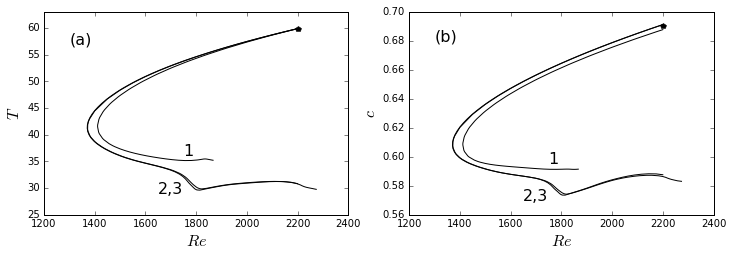
\includegraphics[width=0.9\linewidth]{local_contin.png}}
\caption{Продление модельного порыва в пространстве параметров $(T, c, \Re)$. Изображены зависимость периода изменения решения во времени $T$ и скорости его перемещения вдоль трубы $c$ от числа Рейнольдса $\Re$. Кривые 1, 2 и 3 соответствуют решениям, полученным на различных расчетных сетках. Черные точки соответствует исходному решению, принадлежащему сепаратрисе.}
\label{local_contin_pic}
\end{figure}

Как и на нижней ветви, на верхней решения остаются локализованными в пространстве и меняется во времени периодическим образом, однако они демонстрируют меньшую скорость перемещения вдоль трубы и меньший период изменения во времени. Для них характерна б\'{о}льшая интенсивность пульсаций и вторичных структур. Параметры решения на верхней ветви приближаются к параметрам турбулентного порыва. Это повышает ценность выводов, полученных при изучении решения  с верхней ветви. Если решения с нижней ветви находится на границе области притяжения турбулентного режима течения (на сепаратрисе), то решения с верхней ветви расположены внутри нее и могут участвовать в формировании турбулентного аттрактора\cite{Avila2013}. 

\begin{figure}
\center{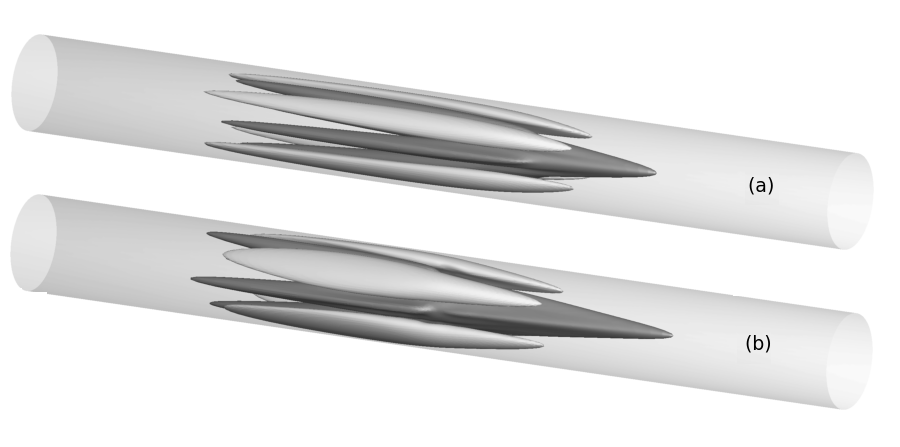
\includegraphics[width=0.9\linewidth]{3D_contin_cmp.png}}
\caption{Среднее поле скорости модельного порыва (1) и решения с верхней ветви при $\Re = 1700$ (2). Темным и светлым тоном выделены поверхности скорости $-0.1$ и $+0.1$ относительно скорости течения Пуазейля. Поток направлен слева направо.}
\label{3D_contin_cmp_pic}
\end{figure}

Для того, чтобы установить параметры расчетной сетки, необходимые для адекватного воспроизведения решений на верхней ветви, решения были найдены на трех различных сетках. Исходная сетка построена при $L_x = 80$ и содержит $512 \times 32 \times 32$ ячеек в продольном, радиальном и угловом направлениях. Также решение было найдено на вдвое более подробной сетке, содержащей $1024 \times 64 \times 64$ ячеек при $L_x = 80$. Для того, чтобы продемонстрировать локализованность решения и его независимость от длины расчетной области, оно было найдено в расчетной области вдвое большей длины, при $L_x = 160$. В этом случае число ячеек в продольном направлении также удвоено, сетка содержит $1024 \times 32 \times 32$ ячеек. На рисунке \ref{local_contin_pic} приведены кривые для решений, полученных на всех трех сетках. Решения, полученные при $L_x = 80$ и $L_x = 160$, обозначенные на рисунке \ref{local_contin_pic} кривыми 2 и 3, практически совпадают друг с другом, что подтверждает пространственную локализованность решения. Характеристики решения, полученного на более подробной стеке, несколько отличаются, причем отличия тем выше, чем дальше решение от исходного. На рисунке \ref{local_contin_pic} подробной сетке соответствует кривая 1. Для более подробного исследования было выбрано решение с верхней ветви при $\Re = 1700$. Хотя при больших $\Re$ решения, полученные на различных сетках, повторяют качественные особенности друг друга, количественные отличия между ними нарастают, и мы не можем гарантировать, что использованных сеток достаточно для адекватного воспроизведения этих решений. Среднее поле скорости выбранного для дальнейшего исследования решения представлено на рисунке \ref{3D_contin_cmp_pic} внизу. Для сравнения изображено также среднее поле скорости модельного порыва вверху. Качественно структура решения не меняется, однако интенсивность полос на верхней ветви выше, чем на нижней. Период по времени выделенного решения можно оценить в $T = 35$, скорость его перемещения вдоль трубы в $c = 0.59$ (скорость перемещения турбулентного порыва вдоль трубы близка к $0.5$). 

Критическое число Рейнольдса, при котором рождается семейство решений, соответствующее модельному порыву, по результатом наших расчетов может быть оценено в $\Re^* = 1400$. В работе \cite{Avila2013} сообщается о близком значении $\Re^* = 1430$. 


\section{Характеристики модельного порыва на верхней ветви}

Продлевая решение, соответствующее модельному порыву, по числу Рейнольдса, удалось достичь точки бифуркации, в которой возникает две ветви решения, и перейти с нижней ветви на верхнюю. Как и модельный порыв, решение с верхней ветви локализовано в пространстве и является условно периодическим по времени, но его характеристики оказываются ближе к характеристикам турбулентного порыва. Параметры выбранного для исследования решение: $\Re = 1700$, $T = 35$, $c = 0.59$. Особенности, выделенные при изучении модельного порыва, могут быть в полной мере обобщены на решение с верхней ветви. 


\begin{figure}
\center{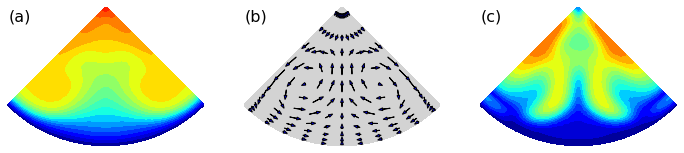
\includegraphics[width=0.9\linewidth]{local_ub_means.png}} 
\center{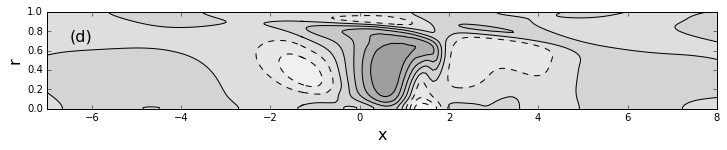
\includegraphics[width=0.9\linewidth]{local_ub_vel1.png}}
\caption{Поле скорости решения с верхней ветви. В сечении, где пульсации достигают наибольшей амплитуды, приведены: (a) --- $V_{x}$, (b) --- $(V_{r}, V_{\theta})$, (c) --- амплитуда $\v_n$; (d) --- мгновенное поле скорости $\v_n$ в сечении $\theta = 0$. }
\label{local_ub_means_pic}
\end{figure}


Как и в модельном порыве, в выделенном решении присутствуют полосы повышенной и пониженной скорости, вытянутые вдоль потока (смотри рисунок \ref{3D_contin_cmp_pic}). При разделении поля скорости решения $\v$ на среднюю $\V = \overline{\v}^t$ и пульсационную $\v_n = \v - \V$ составляющие, полосы попадают с среднюю составляющую движения. Продольная компонента среднего течения $V_x$ изображена на рисунке \ref{local_ub_means_pic}(a). Представлено только одно сечения, однако в других сечениях качественно картина не меняется. Полосы формируются за счет действия продольных вихрей, которые попадают в поперечную компоненту среднего течения $(V_r, V_\theta)$, в том же сечении представленную на рисунке \ref{local_ub_means_pic}(b). Пульсационная составляющая движения $\v_n$ имеет более сложную форму, чем в модельном порыв, однако в первую очередь она представляет собой бегущую вниз по потоку волну. Мгновенное поле скорости пульсационной составляющей движения $\v_n$ в продольном сечении $\theta = 0$ представлено на рисунке \ref{local_ub_means_pic}(d). На рисунке \ref{local_ub_means_pic}(с) представлена амплитуда пульсаций в том же сечении трубы. 


\begin{figure}
\center{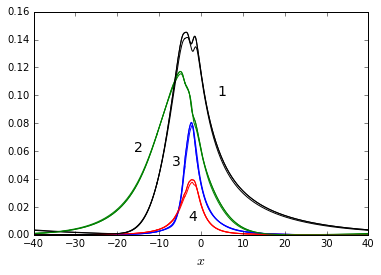
\includegraphics[width=0.6\linewidth]{amp_ub.png}}
\caption{Представлено распределение вдоль трубы амплитуды компонент движения решения с верхней ветви, $\Re = 1700$. Кривая 1 --- отклонение от течения Пуазейля поля скорости $V_{2D}$, кривые 2,3 --- продольная а поперечная компоненты поля скорости $\V_{3D}$, кривая 4 --- средняя по времени $\v_n$. Представлены результаты, полученных на трех расчетных сетках.}
\label{amp_ub_pic}
\end{figure}


На рисунке \ref{amp_ub_pic} изображена средняя по сечению трубы амплитуда различных компонент движения. Как при исследовании модельного порыва, среднее течение разделено на двумерную $\V_{2D} = \overline{\V}^{\theta}$ и трехмерную $\V_{3D} = \V - \V_{2D}$ составляющие. Полосы и продольные вихри попадают в трехмерную составляющую движения. Качественно, распределение интенсивности различных компонент двжиения вдоль трубы в выделенном решении и в модельном порыве совпадают (смотри рисунок \ref{amp_pic}), однако все компоненты движения в выделенном решении имеют большую амплитуду. Интенсивность полосчатого и пульсаций выше примерно в двое. Интенсивность продольных вихрей выше почти в четыре раза. На рисунке \ref{amp_ub_pic} представлены результаты, полученные на трех различных расчетных сетках, описанных в предыдущем разделе. Результаты, полученные на всех сетках, близки друг к другу, что подтверждает достаточность каждой из них для адекватного воспроизведения решения. 



Как в случае модельного порыва, в рассматриваемом случае среднее поле скорости решения на сепаратрисе оказывается линейно неустойчиво. Наиболее быстрорастущее возмущение, возникающее на среднем течении в рамках линеаризованных уравнений \eqref{lin_eq}, воспроизводит форму пульсационной составляющей движения. Оно может быть представлено в виде $\v'_1(x,r,\theta) e^{\lambda_1 t}$. Соответствующий инкремент нарастания оказывается равен $\lambda_1 = 0.014$. В силу относительной однородности среднего течения вдоль трубы, возникающее на нем возмущение близко к бегущей волне. Средняя по времени амплитуда возмущений $\v'_1$ представлена на рисунке \ref{ub_lin_pic}(a) в том же сечении, в котором пульсационная составляющая движения представлена на рисунке \ref{local_ub_means_pic}(c). Поле скорости $\v'_1$ в продольном сечении $\theta = 0$ представлена на рисунке \ref{ub_lin_pic}(b). В этом же сечении приведено мгновенное поле $\v_n$ на рисунке \ref{local_ub_means_pic}(d). Пульсации, возникающие в линейном приближении, $\v_1$, воспроизводят пульсационную составляющую движения $\v_n$, что говорит о том, что $\v_n$ возникает в следствии линейной неустойчивости среднего течения. Отметим, что поле скорости $(V_x, 0, 0)$ оказывается устойчиво к малым возмущениям, соответствующий инкремент затухания приблизительно равен $\lambda = -0.009$. 


\begin{figure}
\center{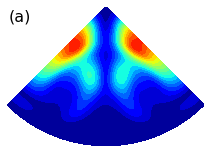
\includegraphics[width=0.3\linewidth]{ub_lin_cs.png} 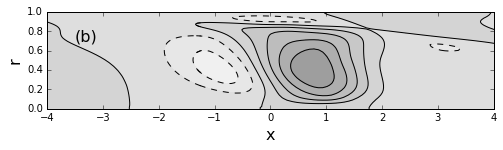
\includegraphics[width=0.6\linewidth]{ub_lin_ls.png}}
\caption{Наиболее быстрорастущее возмущение, возникающее на среднем течении в рамках линеаризованных уравнений \eqref{lin_eq}. Представлены: (a) --- амплитуда пульсаций в поперечном сечении трубы, как на рисунке \ref{local_ub_means_pic}(c); (b) --- мгновенное поле скорости в сечении $\theta = 0$, как на рисунке \ref{local_ub_means_pic}(d). }
\label{ub_lin_pic}
\end{figure}

Полосы повышенной и пониженной скорости возникают вследствие действия стационарных продольных вихрей. 
Механизм образования продольных вихрей в решении с верхней ветви и в модельном порыве также совпадают. На рисунке \ref{ub_OXgen_pic}(a) приведен квадрат средней продольной завихренности $\Omega_x^2$ в одном сечении трубы. Его распределение по сечению трубы соответствует паре продольных вихрей, расположенных между полосами повышенной и пониженной скорости. Определяющий вклад в образование $\Omega_x^2$ дают слагаемые \eqref{time_OXgen_terms}. Их вклад представлен на рисунке \ref{ub_OXgen_pic}(b). Вклад других слагаемых в правой части \eqref{time_OX_eq}, представленный на рисунке \ref{ub_OXgen_pic}(с), существенного влияния на форму продольных вихрей не оказывает. Также на рисунке \ref{ub_oxgen_lines_pic}(a) изображено распределение $\Omega_x^2$ и слагаемых, отвечающих за его формирование, на прямой, проходящей через область, занятую положительным вихрем. Он также подтверждает представления о том, что за образование продольных вихрей ответственно слагаемое \eqref{time_OXgen_terms}. Можно также отметить, что кривые 2 и 3 на рисунке \ref{ub_oxgen_lines_pic}(a) повторяют многие особенности друг друга, но с разным знаком, так что при сложении эти особенности пропадут. Это может быть связано с тем, что слагаемые \eqref{time_OXgen_terms} в этом случае не очень точно соответствуют слагаемым, представляющим физический механизм, ответственный за образование продольных вихрей. 
 

\begin{figure}
\center{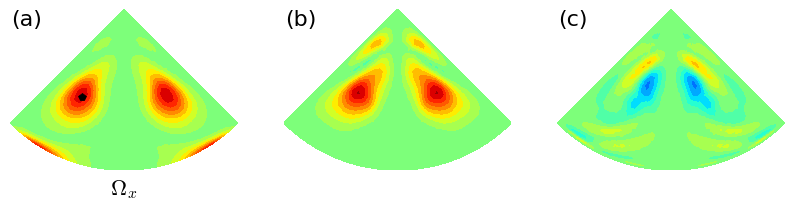
\includegraphics[width=0.9\linewidth]{ub_OXgen_map.png}}
\caption{Для решения с верхней ветви в сечении, где амплитуда пульсаций достигает наибольшего значения, представлены: (a) --- $\Omega_x^2$, (b) и (c) --- вклад в формирование $\Omega_x^2$ со стороны слагаемых \eqref{time_OXgen_terms} и суммы других слагаемых в правой части \eqref{time_OX_eq}. Черная точка на рисунке (a) соответствует прямой, значения на которой представлены на рисунке \ref{ub_oxgen_lines_pic}. Ноль по оси $x$ расположен в сечении, где амплитуда пульсаций достигает максимума.}
\label{ub_OXgen_pic}
\end{figure}

Механизм образования пульсационной составляющей продольной завихренности также сохраняется. На рисунке \ref{ub_oxgen_lines_pic}(b) также, как на рисунке (a), приведено значение амплитуды пульсационной составляющей движения $\overline{\omega'_x\omega'_x}^t$ и вклад в её образование со стороны различных слагаемых в уравнении \eqref{time_ox1_eq}. В области существования продольных вихрей определяющий вклад в образование пульсаций продольной завихренности дает слагаемое \eqref{time_ox1gen_term2}. Его вклад в $\overline{\omega'_x\omega'_x}^t$ изображен кривой 3. Другие слагаемые в правой части \eqref{time_ox1_eq} дают значительно меньший вклад. В частности, слагаемое \eqref{time_ox1gen_terms1}, ответственное за поворот нормальных к стенке вихрей, возникающих в пульсационной составляющей движения, в выделенной области близко к нулю. В этом случае также можно отметить неточность разделения на слагаемых в правой части \eqref{time_ox1_eq} на связанные и несвязанные в механизмом образования пульсаций $\omega'_x$, так как кривые 3 и 4 имеют ряд особенностей, пропадающих при сложении.

\begin{figure}
\center{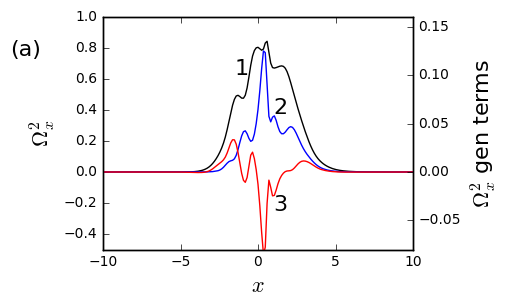
\includegraphics[width=0.5\linewidth]{ub_OXgen_lines.png}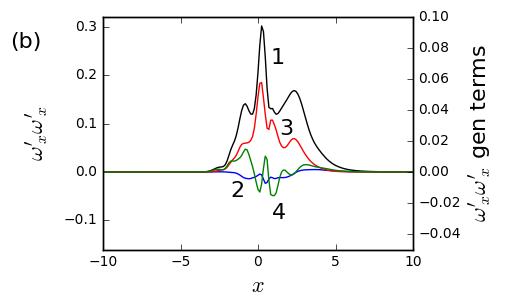
\includegraphics[width=0.5\linewidth]{ub_ox1gen_lines.png}}
\caption{Для решения с верхней ветви на прямой, проходящей через область, занятую положительным вихрем, при $r = 0.6$, $\theta = \pi/10$, представлены: график (a) --- $\Omega_x^2$ (кривая 1) и вклад в его формирование со стороны слагаемых \eqref{time_OXgen_terms} (кривая 2) и других слагаемых в правой части \eqref{time_OX_eq} (кривая 3); график (b) --- $\overline{\omega'_x\omega'_x}^t$ (кривая 1) и вклад в её формирование со стороны слагаемых \eqref{time_ox1gen_terms1} (кривая 2), слагаемого \eqref{time_ox1gen_term2} (кривая 3) и других слагаемых в правой части уравнения \eqref{time_ox1_eq} (кривая~4). Выделенной прямой соответствует черная точка на рисунке \ref{ub_OXgen_pic}(a). Соответствующий рисунок для модельного порыва --- \ref{xline_oxgen_pic}.} 
\label{ub_oxgen_lines_pic}
\end{figure}

Таким образом, весь цикл самоподдержания, выделенный при изучении модельного порыва, может быть обобщен на описанное в разделе решение с верхней ветви. 

\begin{comment}
\begin{figure}
\center{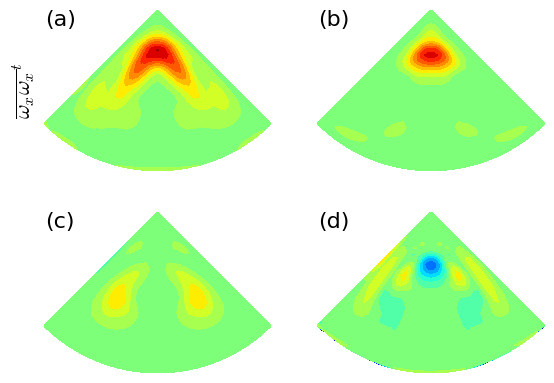
\includegraphics[width=0.6\linewidth]{ub_ox1gen_map.png}}
\caption{Для решения с верхней ветви в сечении, где амплитуда пульсаций достигает наибольшей величины, представлена величина $\overline{\omega'_x \omega'_x}^t$ (график a) и вклад в её формирование со стороны слагаемых \eqref{time_ox1gen_terms1} (график b),  слагаемых  \eqref{time_ox1gen_term2} (график с) и других слагаемых в правой части уравнения \eqref{time_ox1_eq} (график d). }
\label{ub_ox1gen_pic}
\end{figure}
\end{comment}


\section{Характеристики выделенной из турбулентного течения бегущей волны в плоском канале Пуазейля}

Кроме движения жидкости в круглой трубе в работе также было исследованы некоторые случаи движения жидкости в плоском канале Пуазейля. Постановка задачи в этом случае близка к постановке в круглой трубе. В области течения вводится ортогональная системы координат $(x,y,z)$. Ось $x$ направлена вдоль потока, ось $y$ --- по нормали к стенке, ось $z$ --- в трансверсальном направлении. Движение жидкости полагается удовлетворяющем уравнениям Навье-Стокса \eqref{NSeq_Re} и условию несжимаемости \eqref{eq0_Re}. На твердой стенке, расположенной при $y = 0$, ставятся условия прилипания:
\begin{equation}
\v = 0 \text{, при } y = 0
\end{equation}
При $y = 1$ ставится условие проскальзывания, аналогичное условию на оси трубы при дополнительных условиях симметрии в угловом направлении \eqref{sym_eq} и \eqref{per_eq}. Условие проскальзывания имеет вид:
\begin{equation}
\pd{u}{y} = v = \pd{w}{y} = \pd{p}{y} = 0 \text{, при } y = 1
\end{equation}
Здесь $(u,v,w)$ --- компоненты вектора скорости в декартовой системе координат. В качестве единицы длины, таким образом, выступает полуширина канала. Вдоль потока и в трансверсальном направлении ставятся условия периодичности с периодом $L_x$ и $L_z$ соответственно:
\begin{equation}\label{duct_xper_eq}
(\v,p)(x,y,z) = (\v,p)(x+L_x,y,z)
\end{equation}
\begin{equation}\label{duct_zper_eq}
(\v,p)(x,y,z) = (\v,p)(x,y,z+L_z)
\end{equation}
Также, по аналогии с постановкой задачи в трубе, в трансверсальном направлении ставится условие отражения относительно плоскости $z = 0$:
\begin{equation}\label{duct_sym_eq}
(u,v,w,p)(x,y,z) = (u,v,-w,p)(x,y,-z)
\end{equation}
Условия \eqref{duct_zper_eq} и \eqref{duct_sym_eq} могут быть заменены условиями проскальзывания при $z = 0$ и $z = L_z/2$, имеющим вид:
\begin{equation}
\pd{u}{z} = \pd{v}{z} = w = \pd{p}{z} = 0 \text{, при } z = 0, L_z/2 
\end{equation}
Таким образом, расчетная область представляет собой параллелепипед размера $L_x \times 1 \times L_z/2$. Жидкость приводится в движение внешним перепадом давления, определяемым из условия постоянства удельного расхода. В качестве единицы скорости выступает наибольшая скорость в течении Пуазейля. Условие постоянства удельного расхода в безразмерном виде имеет в этом случае вид:
\begin{equation}
\frac{1}{S}\int_{S} u\,dy\,dz = 2/3
\end{equation}
Здесь $S$ --- поперечное сечение трубы и его площадь. Задача поставлена. 


\begin{figure}
\center{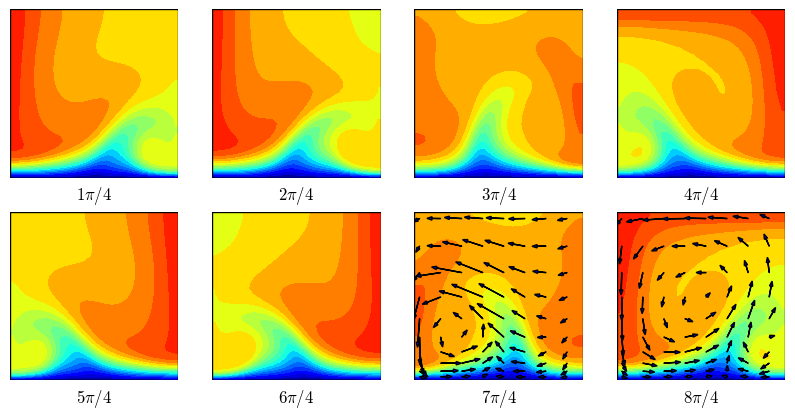
\includegraphics[width=1\linewidth]{duct_turb_map.png}}
\caption{Поле скорости бегущей волны, выделенной из турбулентного течения в плоском канале. Приведена продольная скорости в поперечном сечении в различные фазы течения. На последних двух изображениях приведена также поперечная компонента движения. Твердая стенка находится внизу.} 
\label{duct_turb_tw_pic}
\end{figure}

Было обнаружено, что в расчетной области небольшого размера при небольших значениях числа Рейнольдса турбулентное движение напоминает некоторую бегущую волну. Турбулентное поле скорости оказалось удачным начальным приближением для точной бегущей волны, с которым метод Ньютона сходится. Бегущую волну можно рассматривать, как частный случай условно периодического по времени решения. Для её нахождения может быть использован код, написанный для поиска периодических решений. Параметр $T$, выступающий в качестве периода решения по времени, в данном случае выступает в качестве параметра расчета, не влияющего на результат. Однако отметим, что увеличения значения $T$ позволяет существенным образом сократить число итераций метода решения линейной системы, выполняемого на каждом шаге метода Ньютона. 


\begin{figure}
\center{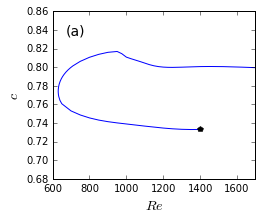
\includegraphics[width=0.45\linewidth]{duct_turb_tw_cf.png}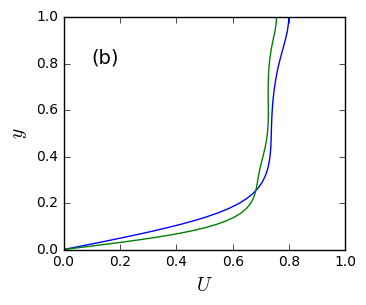
\includegraphics[width=0.45\linewidth]{duct_turb_tw_umean.png}}
\caption{(a) --- зависимость фазовой скорости волны $c$ от числа Рейнольдса $\Re$, черной точкой обозначено исходное решение, принадлежащее верхней ветви; (b) --- средний профиль скорости решения типа бегущей волны с нижней и верхней ветвей, $\Re = 1400$.} 
\label{duct_turb_tw_contin}
\end{figure}


Бегущая волна из турбулентного течения выделена при $L_x = 5$, $L_z = 2$, $\Re = 1400$. Её фазовая скорости равна $c_{tw} = 0.73$. Расчетная сетка, на которой было найдено решение, содержит $64 \times 40 \times 32$ ячеек. Форму бегущей волны позволяет представить рисунок \ref{duct_turb_tw_pic}. На нем изображена продольная скорость в нескольких сечениях трубы, покрывающих один период изменения решения в пространстве (а также во времени). В центре расчетной области около стенки можно выделить полосу замедления, смещающуюся периодическим образом в направлении $z$. Она возникает за счет действия вихрей, расположенных по бокам от полосы замедления в шахматном порядке. Для того, чтобы продемонстрировать существование вихрей, на рисунке \ref{duct_turb_tw_pic} в двух сечения представлена также поперечная компонента скорости. Хотя основные элементы цикла самоподдержания в бегущей волне присутствуют, повторить рассуждения, разработанные при исследовании модельного порыва, для этого решения в полной мере не удается. Амплитуда смещения полосы замедления оказывается слишком велика, так что стандартный метод разделения поля скорости на среднюю и пульсационную составляющие не дает ожидаемого результата. Среднее течение, полученное таким образом, не адекватно воспроизводит форму полос. Метод продления решения по параметру позволяет перевести выделенную бегущую волну к тем значениям параметров, при которых стандартный метод разделения на среднюю и пульсационную составляющие движения дает ожидаемый результат. 




Продлевая выделенную бегущую волну в сторону снижения числа Рейнольдса, удалось достичь точки бифуркации при $\Re = 630$, в которой рождается две ветви решения, и перейти с верхней ветви решения на нижнюю. Зависимость фазовой скорости волны $c_{tw}$ от числа Рейнольдса $\Re$ приведена на рисунке \ref{duct_turb_tw_contin}(a). Для нижней ветви характерны меньшая амплитуда пульсаций, большая фазовая скорость, однако структура решения сохраняется. На рисунке \ref{duct_turb_tw_contin}(b) приведен средний профиль скорости для исходного решения и решения с нижней ветви при том же числе Рейнольдса $\Re = 1400$. Профиль скорости наполненный, на нижней и верхней ветви отличается мало и напоминает профиль скорости в турбулентном потоке. Для дальнейшего анализа выбрано решение, для которого также $\Re = 1400$, $c_{tw} = 0.8$. 

\begin{figure}
\center{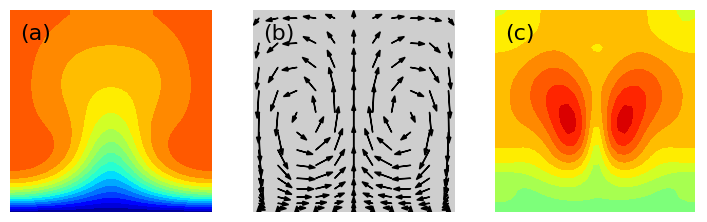
\includegraphics[width=0.9\linewidth]{duct_turb_low_tw_map.png}}
\caption{Нижняя ветвь решения типа бегущей волны, $\Re = 1400$. Приведены: (a) --- средняя продольная компонента скорости $U$, (b) --- средняя поперечная компонента скорости $(V,W)$, (c) --- амплитуда пульсаций $\v_n$.} 
\label{duct_turb_tw_pic}
\end{figure}

Поле скорости $\v$ решения с нижней ветви разделяется на среднюю $\V = \overline{\v}^x$ и пульсационную $\v_n = \v - \V$ составляющие осреднением вдоль трубы. В этом случае среднее поле скорости воспроизводит полосы пониженной и повышенной скорости. Продольная компонента среднего поля скорости $U$ изображена на рисунке \ref{duct_turb_tw_pic}(a). Полоса замедления проходит через центр расчетной области вблизи стенки. Полосы ускорения расположены на границах расчетной области при $z = 0$ и $z = 1$. Полосы возникают с результате действия продольных вихрей. На рисунке \ref{duct_turb_tw_pic}(b) представлена поперечная компонента скорости среднего течения $(V,W)$. Поперечное движение может быть ассоциировано с парой продольных вихрей, расположенных по бокам от полосы замедления. Пульсационная составляющая движения возникает в результате периодического смещения полосы замедления в угловом направлении. Амплитуда пульсаций приведена на рисунке \ref{duct_turb_tw_pic}(c). Они сосредоточены в областях между полосами пониженной и повышенной скорости. Как и в других случаях, пульсационная составляющая движения в этом случае возникает в результате линейной неустойчивости среднего течения. Можно отметить, что и в этом случае поле скорости $(U,0,0)$ оказывается линейно устойчиво, так что пренебрежение поперечным движением качественно меняет характеристики устойчивости среднего течения. 

\begin{figure}
\center{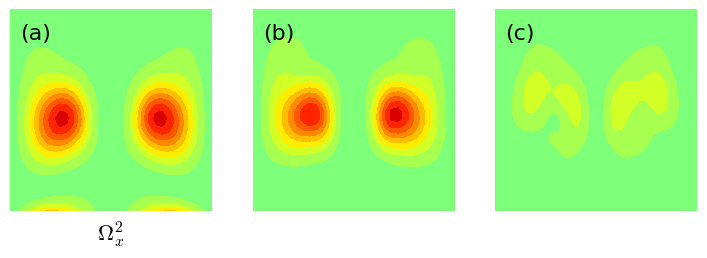
\includegraphics[width=0.9\linewidth]{duct_turb_tw_OXgen.png}}
\caption{Механизм генерации $\Omega_x$ для бегущей волны в плоском канале. Приведено значение $\Omega_x^2$ (a) и вклад в его образование со стороны слагаемых \eqref{OXgen_terms} (b) и суммы других слагаемых в правой части уравнения \eqref{OX_eq} (c).} 
\label{duct_turb_tw_OXgen_pic}
\end{figure}

Выделенное решение позволяет наиболее ярко продемонстрировать механизм образования продольной завихренности. Продольным вихрям соответствуют области повышенной амплитуды стационарной продольной завихренности $\Omega_x$. Квадрат стационарной продольной завихренности изображен на рисунке \ref{duct_turb_tw_OXgen_pic}(a). Форму поля продольной завихренности определяет слагаемое \eqref{OXgen_terms}. Его вклад в $\Omega_x^2$ приведен на рисунке \ref{duct_turb_tw_OXgen_pic}(b). Вклад других слагаемых в правой части уравнения \eqref{OX_eq} представлен на рисунке \ref{duct_turb_tw_OXgen_pic}(с). Их суммарное влияние незначительно, хотя оказывается положительным. Таким образом, нет сомнения, что за образование продольных вихрей ответственны слагаемые \eqref{OXgen_terms}, как и в предыдущих случаях. 

\begin{figure}
\center{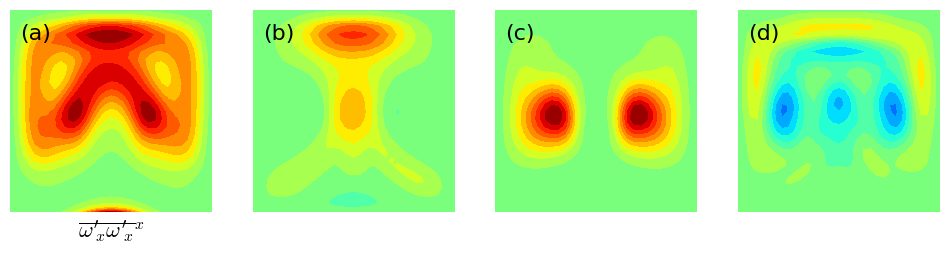
\includegraphics[width=1\linewidth]{duct_turb_tw_ox1gen.png}}
\caption{Механизм генерации $\omega_x'$ для бегущей волны в плоском канале. Приведено значение $\overline{\omega'_x \omega'_x}^x$ (a) и вклад в его образование со стороны слагаемых \eqref{ox1gen_add_terms} (b), \eqref{ox1gen_main_terms} (c) и других слагаемых в правой части уравнения \eqref{ox1_eq} (d).}
\label{duct_turb_tw_ox1gen_pic}
\end{figure}

Образование пульсаций продольной завихренности $\omega'_x$ также происходит в соответствии с выделенным в работе механизмом. Средний вдоль трубы квадрат $\omega'_x$ приведен на рисунке \ref{duct_turb_tw_ox1gen_pic}(a). Как и в предыдущих случаях, на месте продольных вихрей определяющий вклад дает слагаемое \eqref{ox1gen_main_terms}. Его вклад в $\overline{\omega'_x \omega'_x}$ изображен на рисунке  \ref{duct_turb_tw_ox1gen_pic}(c). На рисунке \ref{duct_turb_tw_ox1gen_pic}(b) приведен вклад слагаемого \eqref{ox1gen_add_terms}, связанного с наклоном нормальных к стенке вихрей, возникающих в пульсационной составляющей движения. В отличии от случае модельного порыва, в этом случае на месте продольных вихрей вклад этого слагаемого пренебрежимо мал, что гарантирует, что оно не участвует в образовании продольных вихрей. Вклад других слагаемых, приведенных на рисунке \ref{duct_turb_tw_ox1gen_pic}(с) оказыватеся отрицательным на месте продольных вихрей. Это вновь может говорить о неточности при разделении слагаемых уравнения \eqref{ox1_eq} на связанные и несвязанные с образование продольной завихренности группы.


\section{Характеристики возникающей на сепаратрисе бегущей волны в плоском канале}

В плоском канале может быть найдено решение на сепаратрисе. Метод поиска решения на сепаратрисе в непротяженной расчетной области в постановке, приведенной в предыдущем разделе, позволяет получить бегущую волну, представляющую еще одно семейство решений. Расчеты были выполнены при $L_x = 5$, $L_z = 2.4$, $\Re = 2000$. Возникающая на сепаратрисе бегущая волна в этом случае имеет фазовую скорость $c_{tw} = 0.97$, что близко к максимальной скорости в потоке. Средний профиль её скорости мало отличается от профиля ламинарного течения. Интенсивность пульсаций и движения в поперечной плоскости в этом случае на порядок ниже, чем в бегущей волне, выделенной из турбулентного течения. Тем не менее, структура течения оказывается такой же, как и в других исследованных течениях. В потоке может быть выделена полоса замедления, проходящая через центра расчетной области. Продольная компонента среднего поля скорости $U$ приведена на рисунке \ref{duct_edge_tw_means_pic}(a). В этом случае полоса замедления, как и другие особенности решения, оказывается значительно удалена от твердой стенки. За образование полосы замедления ответственно вторичное течение. Поперечная компонента среднего течения приведена на рисунке \ref{duct_edge_tw_means_pic}(b). Она соответствует паре продольных вихрей, расположенных по бокам от полосы замедления, поддерживающих её существование. Пульсационная составляющая движения сосредоточена в центре канала, и соответствует периодическому смещению области замедления в направлении $z$. Амплитуда пульсаций представлена на рисунке \ref{duct_edge_tw_means_pic}(с). Как и в предыдущих случаях, пульсационная составляющая движения возникает вследствие линейной неустойчивости среднего течения. Кроме того, учет поперечных компонент среднего течения при исследовании его на устойчивость необходим, так как поле скорости $(U,0,0)$ линейной устойчиво. 


\begin{figure}
\center{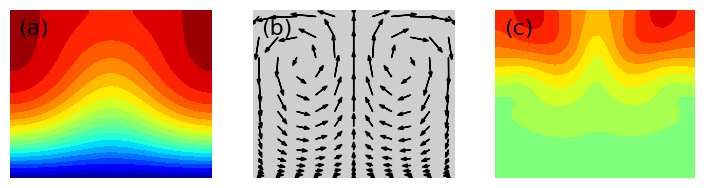
\includegraphics[width=0.9\linewidth]{duct_edge_tw_means.png}}
\caption{Бегущая волна, возникающая на сепаратрисе в плоском канале, $\Re = 2000$. Приведена стационарная продольная составляющая скорости $U$ (a), стационарная поперечная составляющая скорости $(V,W)$ (b) и амплитуда пульсаций $\v_n$ (с).} 
\label{duct_edge_tw_means_pic}
\end{figure}

Механизм образования продольных вихрей в этом случае также согласуется с уже существующими представлениями. Продольные вихри соответствуют областям повышенной концентрации продольной завихренности $\Omega_x$. Квадрат стационарной продольной завихренности $\Omega_x^2$ изображен на рисунке \ref{duct_edge_tw_OXgen_pic}(a). Нет сомнений, что за образование стационарных продольных вихрей ответственны слагаемые \eqref{OXgen_terms}. Их вклад в формирование $\Omega_x^2$ представлен на рисунке \ref{duct_edge_tw_OXgen_pic}(b). Он значительно превосходит по величине вклад других слагаемых, приведенный на рисунке \ref{duct_edge_tw_OXgen_pic}(c), и определяет форму поля $\Omega_x^2$. Механизм образования пульсаций продольной завихренности $\omega'_x$ в этом случае также согласуется с уже разобранными случаями. 

\begin{figure}
\center{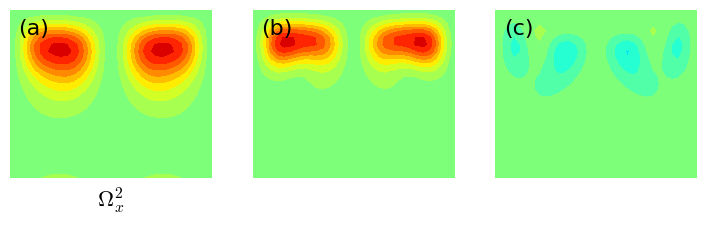
\includegraphics[width=0.9\linewidth]{duct_edge_tw_OXgen.png}}
\caption{Механизм генерации продольных вихрей в бегущей волне, возникающей на сепаратрисе. Приведено значение $\Omega_x^2$ (a) и вклада в его образование со стороны слагаемых \eqref{OXgen_terms} (b) и суммы других слагаемых в правой части уравнения \eqref{OX_eq} (c).}
\label{duct_edge_tw_OXgen_pic}
\end{figure}


\section{Выводы по главе}

В работе, кроме модельного порыва, были найдены и другие инвариантные решения, также допускающие строгое исследование. Их анализ в некоторой степени позволяет установить общность полученных при исследовании модельного порыва результатов. Для всех исследованных решений основные элементы цикла самоподдержания сохраняются, что говорит об их универсальности и позволяет надеяться, что в некотором виде они могут быть найдены в пристенном турбулентном течении непосредственно. 

Продлевая модельный порыв по числу Рейнольдса удалось получить новое условно периодическое локализованное в пространстве решение. Его характеристики оказываются ближе к характеристикам турбулентного порыва, и мы полагаем, что полученные при его исследовании результаты имеют большее отношение к турбулентности. Его анализ показал, что все особенности движения, выделенные при изучении модельного порыва, в полной мере справедливы для найденного решения. Так как оба решения являются представителями одного семейства, можно ожидать, что они воспроизводят общий физический механизм самоподдержания. Тем не менее, полученный результат говорит о том, что механизм самоподдержания сформулирован нами в подходящих терминах; выделенные особенности движения связаны с механизмом самоподдержания существенным образом. 

Также, в плоском канале удалось выделить бегущую волну непосредственно из турбулентного течения. Можно ожидать, что найденное решение воспроизводит особенности, характерные для пристенной турбулентности, хотя её динамика была значительным образом редуцирована наложением условий периодичности в продольном и трансверсальном направлениях. Это может привести к формированию в течении структур, не характерных для свободного турбулентного течения. Важно, что кроме дополнительных условий периодичности, других условий, навязывающих структуру течению, нет. В потоке естественным образом формируется полоса пониженной скорости, расположенная вблизи стенки трубы. Она подвержена значительным по амплитуде колебаниям, что не позволяет, применяя стандартный метод, разделить поле скорости на среднюю и пульсационную части. Однако выделенное решение продлением по числу Рейнольдса было приведено к параметрам, при которых амплитуда пульсаций снижается до уровня, при котором стандартный метод разделения дает желаемый результат. Для полученного таким образом решения справедливы все особенности движения, связанные с числом самоподдержания, выделенные в работе.

Также в плоском канале было была получена бегущая волна, принадлежащая сепаратрисе. Для неё характерна низкая амплитуда вторичного течения и пульсаций, её среднее поле скорости существенно отличается от поля скорости бегущей волны, выделенной в турбулентном течении, однако и в этом решении основные особенности движения, связанные с циклом самоподдержания, выделены. Кроме представленных в главе решений, в работе были получены некоторые другие инвариантные решения. В частности, удалось выделить бегущую волну из турбулентного течения в круглой трубы. Оказалось, что выделенная бегущая волна принадлежит тому же семейству, которому принадлежит бегущая волна, возникающая на сепаратрисе, но если вторя принадлежит нижней ветви, то первая -- верхней. Бегущая волна с верхней ветви повторяет форму бегущей волны, возникающую внутри модельного порыва на верхней ветви. В силу свой избыточности, результаты для неё в главе не приведены. 

Можно отметить, что в ряде случаев есть основания полагать, что слагаемые, отвечающие за формирование продольных вихрей, выделены не точно. Вероятно, уточнить их позволит развитие представлений о физическом механизме, ответственном за этот процесс. Кроме того, метод разделения на среднюю и пульсационную составляющие течения оказался не эффективным при исследовании бегущей волны, выделенной из турбулентного течения. Вероятно, аналогичные сложности могут возникнуть при изучении турбулентного течения непосредственно. Для преодоления возникшего затруднения необходимо разработать новый метод разделения течения на компоненты, пригодный для потоков с большой амплитудой пульсаций.

То обстоятельство, что выделенный при изучении течения в трубе механизм самоподдержания справедлив также и для течений в плоском канале говорит о том, что он связан с кривизной стенки существенным образом. 

Отметим также, что все исследованные решения найдены при условии отражения в трансверсальном направлении. Существует вероятность, что такое условие навязывает некоторую структур течению, не характерную для свободных потоках. 






